
\documentclass[11pt,oneside,a4wide]{report}

\usepackage[ngerman]{babel}
\usepackage{graphicx}
\usepackage[svgnames,table,hyperref]{xcolor}
\usepackage{amssymb}
\usepackage{mathtools}
\usepackage{setspace}
\usepackage{listings}
\usepackage[hyperindex,hidelinks]{hyperref}

\onehalfspacing

\lstdefinestyle{customXML}{
    belowcaptionskip=1\baselineskip,
    breaklines=true,
    frame=L,
    xleftmargin=\parindent,
    language=XML,
    showstringspaces=false,
    basicstyle=\footnotesize\ttfamily,
    keywordstyle=\bfseries\color{green!40!black},
    commentstyle=\itshape\color{purple!40!black},
    identifierstyle=\color{blue},
    stringstyle=\color{orange},
    numbers=left,
    numberstyle=\tiny,
}
\lstdefinestyle{customSQL}{
    belowcaptionskip=1\baselineskip,
    breaklines=true,
    frame=L,
    xleftmargin=\parindent,
    language=SQL,
    showstringspaces=false,
    basicstyle=\footnotesize\ttfamily,
    keywordstyle=\bfseries\color{green!40!black},
    commentstyle=\itshape\color{purple!40!black},
    identifierstyle=\color{blue},
    stringstyle=\color{orange},
    numbers=left,
    numberstyle=\tiny,
}


\newcommand{\HRule}{\rule{\linewidth}{0.5mm}}

\begin{document}

\begin{titlepage}
    \begin{center}

    % Title
    \HRule \\[0.4cm]
    { \huge \bfseries PIM L"osungen\\Praxisteil\\[0.4cm] }
    \HRule \\[1.5cm]

    \textbf{Achtung: Dies ist keine offizielle L"osung!}

    \vfill
    Von:\\
    Dustin Wind


   \vfill
    Zuletzt modifiziert am:\\
    {\large \today}
    \end{center}
\end{titlepage}

%\maketitle

\tableofcontents

%\include{inc/Test/test}

\chapter{PIM Praxisteil 01}

\section{Prozesse und Informationen}

\subsection{p1 Aufgabe S. 4}

Beispielprozess:\\
"`In der Regel wird ein Kunde dann den Kundendienst kontaktieren, wenn er ein subjektiv unl"osbares Problem mit einem Produkt oder einer Dienstleistung hat.
Die Erwartungen an den Kundendienst wird der Kunde mit seinen Erfahrungen abgleichen und bewusst oder unbewusst ein Urteil "uber seine Zufriedenheit oder Unzufriedenheit f"allen."'\\
"`Auch wenn sich das Produkt in einem einwandfreien Zustand befindet und nur ein Bedienungsfehler vorliegt, dann der Kontakt von kunde und Unternehmen "uber Zufriedenheit und ggf. "uber Wiederholungsk"aufe entscheiden.
Ein Kunde wird dann zufrieden sein, wenn sein Problem durch eine effektive und schnelle Unterst"utzung eines Experten behoben wird.
Ein reibungsloser und einfacher Ablauf ist dabei ebenso wichtig wie die kompetente Beratug."'\\

\noindent
Erkl"aren Sie anhand deises Prozesses drei konkrete Ansatzpunkte, wie Informationsmanagement zur Prozessunterst"utzung genutzt werden kann.


\textbf{\#\#\# TODO \#\#\#}\\



\section{Informationsmanagement}

\subsection{p1 Aufgabe S. 8}

F"ur die Entwicklung eines neuen Bibliotheksinformationssystems wird ein konzeptionelles Datenmodell in Form eines Entity-Relationship-Modells ben"otigt.
Folgender Sachverhalt ist abzubilden:\\
B"ucher werden von einem oder mehreren Autoren verfasst.
Jedes Buch ist eindeutig durch seine ISBN gekennzeichnet und erscheint genau in einem Verlag.
Ein Verlag ist durch Name und Ort eindeutig identifiziert.
Von jedem Buch existieren in der Bibliohek ein oder mehrere Exemplare, die von den Lesern ausgeliehen werden k"onnen.
Wird ein Exemplar ausgeliehen, so wird das R"uckgabedatum vermerkt.\\
Erstellen Sie bitte das zugeh"orige ERM.
Modellieren Sie auch die im Text angegebenen Attribute und erg"anzen Sie, wo notwendig, die jeweils identifizierenden Attribute.

\bigskip

\noindent
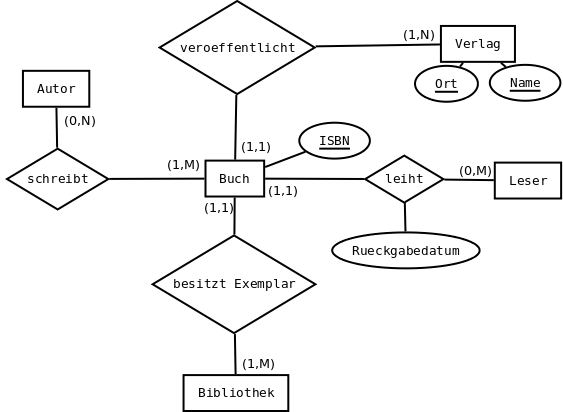
\includegraphics[scale=0.5]{./inc/p1_umlaufgabe}

\subsubsection{p1 Aufgabe S.24}
Ein wesentlicher Aspekt der relationalen Datenmodellierung ist die so genannte Normalisierung.\\
\noindent
$a)$ Erl"autern Sie bitte, welches Ziel mit der Normalisierung verfolgt wird.
Welcher Pahse des Modellierungsprozesses ist die Normalisierung zuzuordnen?\\

\begin{quote}
Um der L"osch-, Einf"uge- und "Anderungs-Anomalie entgegen zu wirken m"ussen Tabellen normalisiert werden.
Das bedeutet, dass alle Redundanzen entfernt werden m"ussen.\\
Die Normalisierung l"asst sich der Feindatenmodellierung zuordnen.
\end{quote}

\noindent
$b)$ Nennen und begr"unden Sie bitte, in welcher Normalform sich die folgende Tabelle befindet.\\

\begin{quote}
Die Tabelle "`Studenten\_zu\_Pr"ufungen"' ist in der \textbf{ersten Normalform}.
Sie ist in der ersten Normalform weil \textbf{jede Eigenschaft nur einen Eigenschaftswert} enth"alt.\\
Die Tabelle ist jedoch nicht in der zweiten Normalform, da Nicht-Schl"usselattribute abh"angig von einer echten Teilmenge der Schl"usselkandidaten ist.
\end{quote}

\noindent
$c)$ "Uberf"uhren Sie die Tabelle aus Teilaufgabe $b)$ bitte in die n"achsth"ohere Normalform.\\


\rowcolors{1}{LightGray}{White}
\begin{tabular}{ l l }
    \hline
    \rowcolor{LightSlateGrey}
    \textbf{Matrikelnummer} & \textbf{Studentname} \\
    111111                  & M"uller\\
    333333                  & Schmidt\\
\end{tabular}

\vspace{1cm}

\begin{tabular}{ l l }
    \hline
    \rowcolor{LightSlateGrey}
    \textbf{Pr"ufungsnummer}    & \textbf{Pr"ufungsname}\\
    6144                        & Prozess- und Informationsmanagement\\
    2377                        & E-Procurement\\
\end{tabular}

\vspace{1cm}

\begin{tabular}{ l l l }
    \hline
    \rowcolor{LightSlateGrey}
    \textbf{Matrikelnummer} & \textbf{Pr"ufungsnummer}  & \textbf{Note}\\
    111111                  & 6144                      & 1,0\\
    111111                  & 2377                      & 1,3\\
    333333                  & 6144                      & 2,0\\
\end{tabular}




\chapter{PIM Praxisteil 02}

\section{Datenmanagement}

\subsection{p2 Aufgabe S. 23}

Stellen Sie bitte da, wie ein SQL-SELECT-Statement aufgebaut ist und welchen Operationen aus der Relationentheorie die einzelnen Bestandteile entsprechen.
\begin{itemize}
    \item SELECT $A_1$, \dots, $A_n$\\
    $\Rightarrow$ Projektion
    \item FROM $R_1$, \dots, $R_n$\\
    $\Rightarrow$ Kartesisches Produkt
    \item WHERE Pr"adikat($R_1$, \dots, $R_n$)\\
    $\Rightarrow$ Selektion
\end{itemize}

\subsection{p2 Aufgabe S. 24}

\lstset{style=customSQL}
\begin{lstlisting}
SELECT  BestellNr, Auslieferdatum, Name
FROM    Bestellung AS b
        JOIN Kunde AS k ON b.KundenNr = k.KundenNr
WHERE   b.Bezahlt = 0
;
\end{lstlisting}

Alternativ ohne "`JOIN"':
\lstset{style=customSQL}
\begin{lstlisting}
SELECT  BestellNr, Auslieferdatum, Name
FROM    Bestellung
        , Kunde
WHERE   Bestellung.KundenNr = Kunde.KundenNr
        AND Bestellug.Bezahlt = 0
;
\end{lstlisting}


\subsection{p2 Aufgabe S. 26}

\lstset{style=customSQL}
\begin{lstlisting}
SELECT      g.Bezeichnung AS Gemuese
            , COUNT(*) AS Anzahl
FROM        Patient AS p
            JOIN ESSEN AS e ON p.ID = e.PatientenID
            JOIN Gemuese g ON g.ID = e.GemueseID
WHERE       p.Schweregrad = 'schwer'
GROUP BY    g.GemueseID
;
\end{lstlisting}
Alternativ ohne "`JOIN"':
\lstset{style=customSQL}
\begin{lstlisting}
SELECT      Gemuese.Bezeichnung AS Gemuese
            , COUNT(*) AS Anzahl
FROM        Patient
            , Essen
            , Gemuese
WHERE       Patient.ID = Essen.ID
            AND Gemuese.ID = Essen.GemueseID
            AND Patient.Schweregrad = 'schwer'
GROUP BY    Gemuese.GemueseID
;
\end{lstlisting}

\subsection{p2 Aufgabe S. 27}

\lstset{style=customSQL}
\begin{lstlisting}
INSERT INTO ESSEN (PatientenID, GemueseID, Datum)
VALUES  (
    (
        SELECT  ID
        FROM    Patient
        WHERE   Vorname = 'Mathilda'
                AND Name = 'Natter'
    ) -- get the ID for the given patient
    ,
    (
        SELECT  ID
        FROM    Gemuese
        WHERE   Bezeichnung = 'Sprossen'
    ) -- get the ID for the given vegetable
    '2.06.2011')
;
\end{lstlisting}


\section{Datawarehouse}

\subsubsection{p2 Aufgabe S. 57}
Data Warehouses erm"oglichen im Allgemeinen so genannte Roll-Ups.
Dabei wird die Aggregationsstufe der Daten immer weiter erh"oht, so dass die Betrachtung von den Details ausgehend stetig globaler wird.
Zur Unterst"utzung dieser Operation wurde die Datenmanipulationssprache SQL um das "`Group By Rollup"'-Statement erweitert.\\\noindent
Gegeben sei die Tabelle \textit{Verk"aufe}:\\

\begin{tabular}{l l l l l}
    \rowcolor{LightSlateGray}
    \textbf{Produkt}    & \textbf{Gebiet}   & \textbf{Quartal}  & \textbf{Monat}    & \textbf{Umsatz}\\
    CD  & D & 1/14  & Jan   & 27\\
    CD  & D & 1/14  & Feb   & 13\\
    CD  & D & 1/14  & Mar   & 12\\
    VCR & D & 1/14  & Jan   & 19\\
    VCR & D & 1/14  & Mar   & 21\\
    CD  & F & 1/14  & Jan   & 20\\
    CD  & F & 1/14  & Mar   & 18\\
    VCR & F & 1/14  & Feb   & 23\\
\end{tabular}

\bigskip

\noindent
Bestimmen Sie bitte auf Basis dieser Tabelle das Ergebnis der folgenden Abfrage:\\

\lstset{style=customSQL}
\begin{lstlisting}
SELECT          Produkt, Gebiet, Quartal
                , SUM(Umsatz) AS Gesamtumsatz
FROM            Verkaeufe
WHERE           Quartal = '1/14'
GROUP BY ROLLUP ( Quartal, Produkt, Gebiet)
;
\end{lstlisting}

\bigskip

\rowcolors{0}{White}{White}
\begin{tabular}{ l l l l }
    \textbf{Produkt} & \textbf{Gebiet} & \textbf{Quartal} & \textbf{Gesamtumsatz}\\\hline
    \rowcolor{NavyBlue!10}  CD  & D & 1/14  & 52\\
    \rowcolor{NavyBlue!10}  VCR & D & 1/14  & 40\\
    \rowcolor{NavyBlue!10}  CD  & F & 1/14  & 38\\
    \rowcolor{NavyBlue!10}  VCR & F & 1/14  & 23\\\hline
    \rowcolor{NavyBlue!20}  CD  &   & 1/14  & 90\\
    \rowcolor{NavyBlue!20}  VCR &   & 1/14  & 63\\\hline
    \rowcolor{NavyBlue!30}      &   & 1/14  & 153\\
\end{tabular}

\subsection{p2 Aufgabe S. 60}
Der Chef des Ski- und Snowboardverleihs Winterhart speichert den Verleih seiner Ausr"ustung in einem Data Warehouse.
Mithilfe von OLAP m"ochte er einen besseren "Uberblick dar"uber bekommen, welche Ausr"ustung an welchen Standorten in welchen Zeitr"aumen verliehen wird.\\

\noindent
$a)$ In einem Buch hat der Chef des Ski- und Snowboardverleihs etwas "uber die OLAP-Operationen Slice, Dice und Roll-Up gelesen.
Erl"autern Sie bitte allgemein das Ziel dieser OLAP-Operatoren.

\begin{quote}
    \textbf{Slice/Dice}\\
    Ebenen (Slices) bzw. Unterw"urfel (Dices) werden in das Blickfeld des Betrachters geholt.\\
    \textbf{Drill-Down/Roll-Up}\\
    Stufenweise detaillierte bzw. aggregiertere Betrachtungsweise.\\
\end{quote}

\noindent
$b)$ Der Chef des Ski- und Snowboardverleihs zeigt Ihnen folgenden Ausschnitt aus seiner Datawarehouse-Tabelle "`Verleih"':\\

\rowcolors{0}{LightGray}{White}
\begin{tabular}{ l l l l }
    \rowcolor{LightSlateGrey}
    \textbf{Ausr"ustung} & \textbf{Standort} & \textbf{Monat} & \textbf{Anzahl}\\
    Ski         & Oberstdorf                & 12/2010   & 840\\
    Ski         & Garmisch-Partenkirchen    & 12/2010   & 960\\
    Ski         & Oberstdorf                & 01/2011   & 530\\
    Ski         & Garmisch-Partenkirchen    & 01/2011   & 420\\
    Snowboard   & Oberstdorf                & 12/2010   & 900\\
    Snowboard   & Garmisch-Partenkirchen    & 12/2010   & 950\\
    Snowboard   & Oberstdorf                & 01/2011   & 600\\
    Snowboard   & Garmisch-Partenkirchen    & 01/2011   & 550\\
\end{tabular}

\bigskip

\noindent
Bitte zeigen Sie auf welche Ergebnisse der Chef des Ski- und Snowboardverleihs erh"alt, wenn er folgendes SQL-Statement formuliert.\\

\lstset{style=customSQL}
\begin{lstlisting}
SELECT                  Ausruestung
                        , Monat
                        , Sum(Anzahl) AS Gesamtanzahl
FROM                    Verleih
GROUP BY GROUPING SETS  ((Ausruestung, Monat)
                            , (Ausruestung)
                            , ())
;
\end{lstlisting}

\bigskip

\rowcolors{0}{LightGrey}{White}
\begin{tabular}{ l l l }
    \rowcolor{LightSlateGray}
    \textbf{Ausr"ustung} & \textbf{Monat} & \textbf{Gesamtanzahl}\\
    Ski         & 12/2010   & 1800\\
    Ski         & 01/2010   & 950\\
    Snowboard   & 12/2011   & 1850\\
    Snowboard   & 01/2011   & 1150\\
    Ski         &           & 2750\\
    Snowboard   &           & 3000\\
\end{tabular}




\section{Document Type Definitions (DTD)}


\subsection{Aufgabe}
Deklarieren Sie eine Attributliste f"ur das Elemente "`Catalog\_Structure"'.
Diese Attributliste soll das Attribut "`type"' beinhalten, welches vom Typ Aufz"ahlung ist und die Werte "`root"', "`node"' oder "`leaf"' annehmen kann.
Das Attribut soll als "`required"' definiert werden.\\

\lstset{style=customXML}
\begin{lstlisting}
<!ATTLIST Catalog_Structure type (root|node|leaf) #REQUIRED>
\end{lstlisting}

\subsection{Aufgabe}
F"ugen Sie dem Element BMECat ein weiteres Attribut namens "`note"' hinzu und deklarieren Sie es als optional.\\

\lstset{style=customXML}
\begin{lstlisting}
<!ELEMENT BMECat (Header,(T_New_Catalog,note)?)>
\end{lstlisting}


\subsection{Aufgabe}

Formulieren Sie eine Document Instance, die auf die DTD "`BMECat.dtd"' referenziert und folgende Inhalte Abbildet:\\
Es handelt sich um die Beschreibung des Katalogs "`Bademoden 2005"'.
Der Katalog tr"agt die ID 200345 und liegt in deutscher Sprache in der Version 1.0 vor.

\lstset{style=customXML} % given DTD
\begin{lstlisting}
<!ELEMENT BMECat (Header, T_New_Catalog)>
<!ATTLIST BMECat version CDATA #FIXED "1.2">
<!ELEMENT Header (Catalog, Buyer, Supplier)>
<!ELEMENT Catalog (Language, Catalog_Id, Catalog_Version, (Catalog_Name)?, (Currency)?>
<!ELEMENT Language (#PCDATA)>
<!ELEMENT Catalog_Id (#PCDATA)>
<!ELEMENT Catalog_Version (#PCDATA)>
<!ELEMENT Catalog_Name (#PCDATA)>
<!ELEMENT Currency (#PCDATA)>
\end{lstlisting}

\lstset{style=customXML}
\begin{lstlisting}
<!DOCTYPE BMECat "BMECat.dtd">
<? xml version='1.0' encoding="UTF-8"?>
<BMECat version='1.2'>
    <Header>
        <Catalog>
            <Language>deutsch</Language>
            <Catalog_Id>200345</Catalog_Id>
            <Catalog_Version>1.0</Catalog_Version>
        </Catalog>
    </Header>
</BMECat>
\end{lstlisting}




\subsection{Aufgabe}
Aufgrund welcher Fehler ist das folgende XML-Dokument nicht wohlgeformt?

\lstset{style=customXML}
\begin{lstlisting}
<?xml version="1.0" encoding="ISO-8859-1"?>
<!DOCTYPE order SYSTEM "order.dtd">
<order Id="234">
    <item>
        <title>XML and Java</title>
        <price currency="EUR">100.0</price>
        <quantity>1
    </item>
    <cardinfo>
        <name>Your Name<name/>
        <expiration>04/2002</expiration>
        <number></cardinfo>5283830462320010</number>
</order>
\end{lstlisting}

Korrigiertes XML:
\lstset{style=customXML}
\begin{lstlisting}
<?xml version="1.0" encoding="ISO-8859-1"?>
<!DOCTYPE order "order.dtd">
<order Id="234">
    <item>
        <title>XML and Java</title>
        <price currency="EUR">100.0</price>
        <quantity>1</quantity>
    </item>
    <cardinfo>
        <name>Your Name</name>
        <expiration>04/2002</expiration>
        <number>5283830462320010</number>
    </cardinfo>
</order>
\end{lstlisting}


\subsection{Aufgabe}

Die Innova AG beabsichtigt, den Austausch von Rechnungsdaten mit ihren Kunden per XML abzuwickeln.
Der Entwurf einer entsprechenden Document Type Definition (DTD) f"ur die zuk"unftigen Rechnungsformulare ist bereits vorhanden:

\subsubsection{Aufgabe a)}
Die Elementtypen Ansprechpartner und Land sollen optional deklariert werden.
Auspr"agungen des Elementtyps Rechnungsposition k"onnen in einer Dokument-Instanz ein oder mehrmals vorkommen.\\

\lstset{style=customXML}
\begin{lstlisting}
<!ELEMENT Kunde (Kundennummer, Firmenname, (Ansprechpartner)?, Adresse)>
<!ELEMENT Rechnungsdaten (Rechnungsnummer, Rechnungsdatum, (Rechnungsposition)*, Nettogesamtbetrag, Mehrwertsteuer, Bruttogesamtbetrag)>
\end{lstlisting}

\subsubsection{Aufgabe b)}
Deklarieren Sie bitte ein Element vom Typ Bankverbindung mit Zeichendaten als Inhalt und ordnen Sie es an passender Stelle in das Inhaltsmodell der DTD ein.\\
\lstset{style=customXML}
\begin{lstlisting}
<!ELEMENT Bankverbindung (#PCDATA)>
<!ELEMENT Kunde (Kundennummer, Firmenname, (Ansprechpartner)?, Adresse, Bankverbindung)>
\end{lstlisting}

\subsubsection{Aufgabe c)}
Da die Bankverbindungen f"ur einen l"angeren Zeitraum konstant bleibt, schlagen Sie vor, ein Entity vom Typ BV mit dem Inhalt "`Innova AG, Kto-Nr. 1234567, BLZ 76959191, Stadtsparkasse Nuernberg"' in der DTD zu deklarieren.
Bitte formulieren Sie die Entsprechende Entitytypdeklaration.\\

\lstset{style=customXML}
\begin{lstlisting}
<!ELEMENT BV (#PCDATA)>
\end{lstlisting}

\subsubsection{Aufgabe d)}
F"ur jede Rechnung sollen jeweils Bearbeiter und Bearbeitungsstatus zugeordnet werden k"onnen.
Dies kann durch Einf"uhrung von entsprechenden Attributen realisiert werden.
Definieren Sie bitte die erforderlichen Attribute und ordnen Sie diese dem Wurzelelement des Dokuments zu.
Das Attribut Bearbeiter ist als \#REQUIRED zu deklarieren.
Das Attribut Bearbeitungsstatus kann die Werte "`ungeprueft"', "`geprueft"', oder "`freigegeben"' annehmen un dhat standardm"a"sig den Wert "`ungeprueft"'.

\lstset{style=customXML}
\begin{lstlisting}
<!ATTLIST Rechnung Bearbeiter CDATA #REQUIRED>
<!ATTLIST Rechnung Bearbeitungsstatus ("ungeprueft"|"geprueft"|"freigegeben") #FIXED "ungeprueft">
\end{lstlisting}

\subsection{Aufgabe}
Ein bekannter N"urnberger Jugendsachbuchverlag m"ochte seinen content mehrfach nutzen (Web und Print). 
Sie empfehlen dem Verlag, die Inhalte medienunabh"angig in XML-Dokumenten abzulegen.
Eine DTD beschreibt die Struktur von XML-Dokumentinstanzen.
Bitte erstellen Sie mithilfe der folgenden Angaben eine DTD zur Strukturierung eines mehrfach nutzbaren Artikels:\\

"`Jeder Artikel hat eine "Uberschrift, einen Textk"orper, einen Autor und ein Erstellungsdatum.
Der Autor hat immer einen Vor- und einen Nachnamen, optional kann ein akademischer Titel angegeben werden.
Der Textk"orper besteht aus mindestens einem Absatz.
Jeder Artikel enth"alt auch einen Copyrightvermerk.
Da dieser meistens gleich ist, soll f"ur den Inhalt ein Entity mit dem Inhalt 'Tossleff Jugendsachbuch AG' vordefiniert werden.
Da nicht jeder Artikel sowohl online als auch offline verf"ugbar sein soll, wird ein entsprechendes Attribut ben"otigt (z.B. "`type"'), das den Inhalt "`web"', "`print"' oder "`multichannel"' haben kann.
Dieses Attribut ist nicht optional."'\\

\lstset{style=customXML}
\begin{lstlisting}
<!ELEMENT Artikel (Ueberschrift, Textkoerper, Autor, Erstellungsdatum, Copyright)>
    <!ELEMENT Ueberschrift (#PCDATA)>
    <!ELEMENT Textkoerper ((Absatz)+)>
        <!ELEMENT Absatz (#PCDATA)>
    <!ELEMENT Autor ((Vorname), (Nachname), (Titel)?)>
        <!ELEMENT Vorname (#PCDATA)>
        <!ELEMENT Nachname (#PCDATA)>
        <!ELEMENT Titel (#PCDATA)>
    <!ELEMENT Erstellungsdatum (#PCDATA)>
    <!ENTITY Copyright "Tossleff Jugendsachbuch AG">
    <!ATTLIST Artikel type ('web'|'print'|'multichannel' #REQUIRED)>
\end{lstlisting}



































































\section{XQuery}

\subsection{Aufgabe}

\lstset{language=PHP}
\begin{lstlisting}
for $schuh in doc("Sportschuhkatalog.xml")/Sportschuhkatalog/Sportschuh

where $schuh/Basisfarbe = "rot"

return $schuh/ID
\end{lstlisting} %$ // correct the syntaxhighlithing within vim


\subsection{Aufgabe}

\textbf{\#\#\# TODO \#\#\#}\\
// Layoutorientierte vs. contentorientierte Verfahren zur Erstellung von Medienprodukten

\subsection{Aufgabe}

\textbf{\#\#\# TODO \#\#\#}\\
// Precision + Recall von Suchmaschinen


\subsection{Aufgabe}

\textbf{\#\#\# TODO \#\#\#}\\
// Precision + Recall von Suchmaschinen





\end{document}



